


\subsubsection{Training Loop}
\label{sec:Method:Learning:TrainingLoop}
The training loop for the proposed model is presented in the algorithm below:

\begin{algorithm}[H] 
\caption{Training of the Stepwise Constant Velocity Model. Return the log-likelihood of events.}
\label{alg:TrainingLoop}
\begin{algorithmic}%[1]
\Require{Batch of entire dataset of event tuples $(u_i, v_i, t_i)$, for $i = 1,\dots,n$. Also number of velocities, steps $s = 1,\dots,m$, to fit.} 
\Ensure{log-likelihood $\ell$}
\Statex

\State {$EventIntensity = 0$}
\State {$NonEventIntensity = 0$}

\For{m}                    
    \State {$EventIntensity_s = 0$}
    \For{$u_{s,i}, v_{s,i}, t_{s,i}$} 
        \State {$EventIntensity_s \mathrel{+}= \beta - ||z_u(t) - \z_v(t)||_2^2$}
    \EndFor
    \State {$EventIntensity \mathrel{+}= EventIntensity_s$}
\EndFor
\\
\For{m} 
    \State {$NonEventIntensity_s = 0$}
    \For{$NodePair: u,v$} 
        \State {$NonEventIntensity_s \mathrel{+}= integral(u, v, t_0, t_n, n)$}
    \EndFor
    \State {$NonEventIntensity \mathrel{+}= NonEventIntensity_s$}
\EndFor
\\
\State {$LogLikelihood = - EventIntensity - NonEventIntensity$}
\State \Return {$LogLikelihood$}
\EndFunction
\end{algorithmic}
\end{algorithm}
NOT COMPLETELY FINISHED, BUT THE FINAL PART OF THIS SECTION NONTHELESS.









\begin{figure}[H]
    \centering
    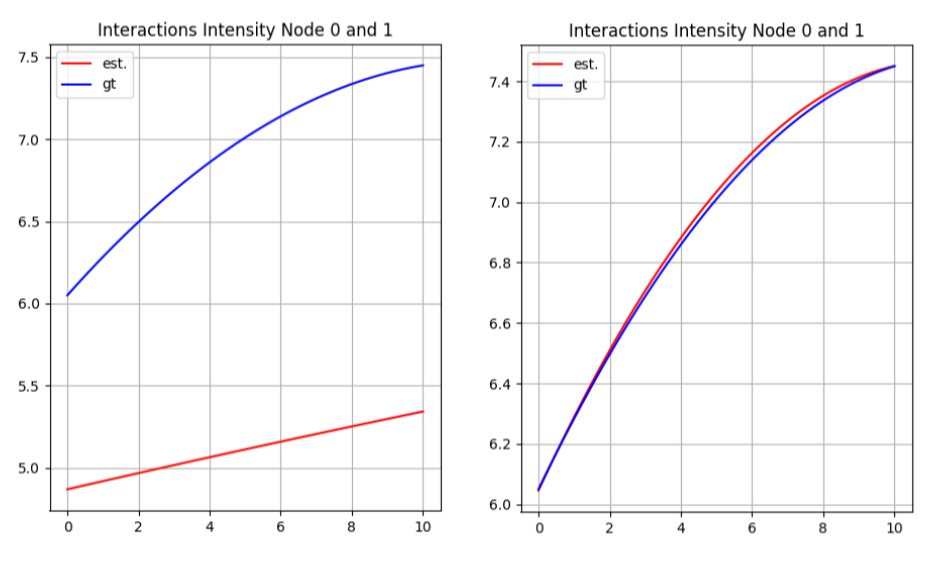
\includegraphics[width=\textwidth]{0_images/5vs5000epochs.png}
    \caption{Example of Interaction Intensity Comparison: Interaction intensity (y-axis) from time 0 to 10 (x-axis) between nodes 0 and 1 for a given system. Blue is the ground truth model and red is the trained model. Left compares intensities after training the model for 5 epochs, right after training for 5000 epochs.}
    \label{fig:5vs5000epochs}
\end{figure}